\chapter{DESCRIPTION OF MY WORK}
\label{chap:five}
The following chapter discusses the process of creating an interactive visualization tool, choosing the right frameworks, and using them to create new solutions to explore flow cytometry data. The importance of skills in various fields such as data science, statistics, design, and software development is highlighted. Architecture of final solution is described.

\section{Requirements for developing an visual analysis tool}
\label{sec:req}
While each of the frameworks described in \ref{chap:four} has their own merit and their own pitfalls, the overall performance of a tool depends on user's requirements, expectations, and skills. Building data visualization tools is based on a variety of fields, such as data science, statistics, design, and software development. 

Skills from the area of design are understanding the use of color, typography, and layout, which can all help communicate insights about the data clearly to the end user. 

From software development side of things, one has to be able to use a language of choice to enable the implementation of concepts from the past paragraph, and also broad knowledge of available tools and libraries is welcome. The implementation does not have to be as straightforward as it would seem at first glance, so strong problem-solving skills are welcome, as is orientation to detail. 

\section{Selected Technologies and Architecture}
\label{sec:selected_technologies}
Two frameworks described in \ref{chap:four}, namely Streamlit \ref{sec:streamlit} and Dash \ref{sec:dash}, were chosen as frameworks in which the visualization tool would be developed. The rich communities of both frameworks provide a deep pool of knowledge, and promise support from the creators and future development. Both have proven a tool worthy of the task of visualizing and exploring a flow cytometry dataset. 

The tool consists of several layers as described below.
\begin{figure}[h!]
    \centering
    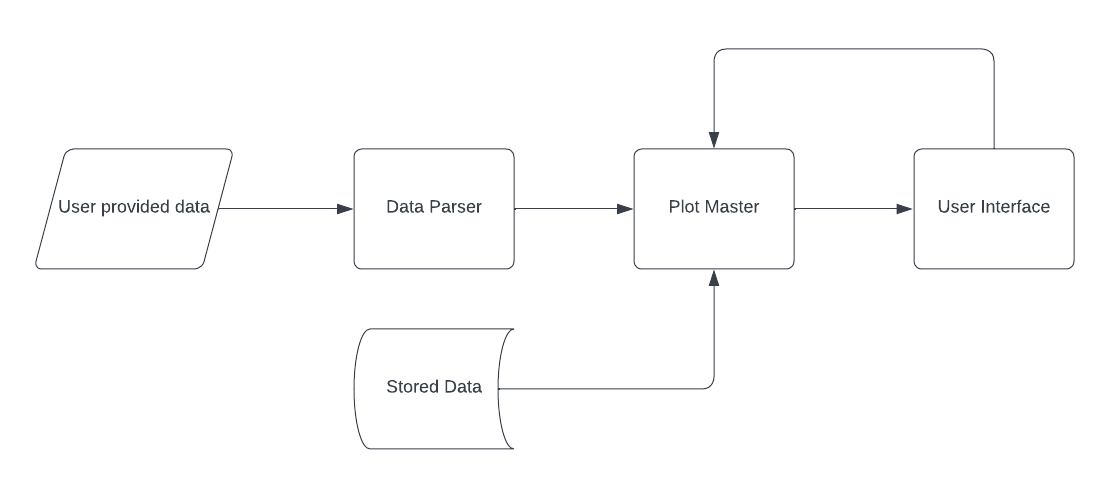
\includegraphics[width=0.9\textwidth]{Figures/Flowchartex1.png}
    \caption{Flowchart}
    \label{fig:flowchart}
\end{figure}

\subsection{Data Parsing}
\label{sec:data-parsing}
A custom parsing solution was developed to read and translate input data necessary for dendrogram visualization. The input data is expected to be put in the "user\textunderscore data" folder. Three files are expected:
\begin{itemize}
    \item heights.csv
    
    Heights refer to the height attribute used in dendrograms. The height attribute represents the heights of individual nodes in the dendrogram in the form of a numeric vector. Each element of the vector is tied to a specific node. Each of the elements measures height from the beginning. 
    
    \item merge.csv

    Merge is a 2D matrix that describes the hierarchical clustering solution. Each row is a description of two components used in a merger. Positive values indicate individual observations (leaf nodes) and negative values indicate clusters formed in previous mergers. More on the iterative process of hierarchical clustering can be read in \ref{sec:hierarchicalclustering}.
    
    \item order.csv

    Order is a vector of positive integers that describes the order in which observations were merged together. The indexing of the data in order.csv is expected to start at 1, as DataParser subtracts 1 from each element to match Python's indexing, which starts at 0. Order is useful for data visualization as it helps the program navigate the easiest way to plot leaves without creating unnecessary cross-overs. 
\end{itemize}

It is also possible to add a fourth file:
\begin{itemize}
    \item labels.csv
    
    Labels is an optional file that should contain a 1D matrix of strings describing each of the datapoints. However, in case the user does not have labels available, mock labels will be provided assigning each element a value from 0 to len(data). 
\end{itemize}

The file format was inspired by the output of R's hclust function.

One file that is not used in plotting the dendrogram is:
\begin{itemize}
    \item data.csv
    
    The data.csv should contain a matrix in which columns represent features and rows represent each of the samples. It can either be raw or preprocessed data. This file is used to plot data represented in dendrogram with the aim to make data exploration more accessible.
\end{itemize}

\subsection{Data Plotting}
\label{sec:data-plotting}
The main component responsible for plotting the data is PlotMaster. The PlotMaster expects data which has been preprocessed by the DataParser. This architecture was selected for merits of having each of the processes split, making it easy to build prototypes in multiple front-end solutions. A well ordered application reduced confusion should the user need to understand anything from the code. 

The PlotMaster leverages Plotly (for deeper description of Plotly see \ref{sec:plotly}) graphing library under the hood. It is designed to help the user explore the data in a visual way. The ability to pan, zoom in, zoom out, or save the plot as .png file is integrated into Plotly. 

There are four types of plots offered by the PlotMaster:
\begin{itemize}
    \item Dendrogram

    Dendrogram is a tree representation of hierarchical clustering as described in \ref{sec:hierarchicalclustering}. The user can interact with the dendrogram by setting color threshold. Color threshold is an integer which is responsible for the height in which clusters are set to different colors, helping the user detect them visually. 
    \begin{figure}[h!]
        \centering
        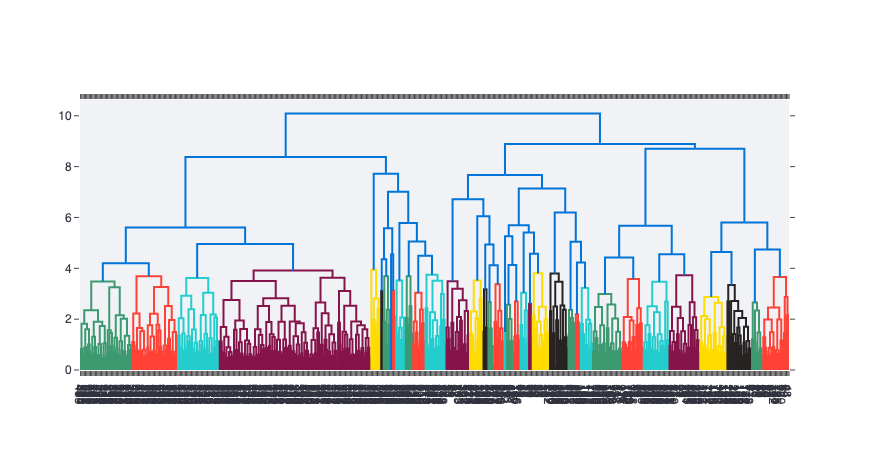
\includegraphics[width=0.9\textwidth]{Figures/dendrogramex.png}
        \caption{Dendrogram}
        \label{fig:dendrogram}
    \end{figure}

    \item Heatmap

    Heatmap is a way to visualize data quantity in color dependent manner as described in \ref{sec:hierarchicalclustering}. The user can specify which features they would like to plot in the available heatmap. 
    \begin{figure}[h!]
        \centering
        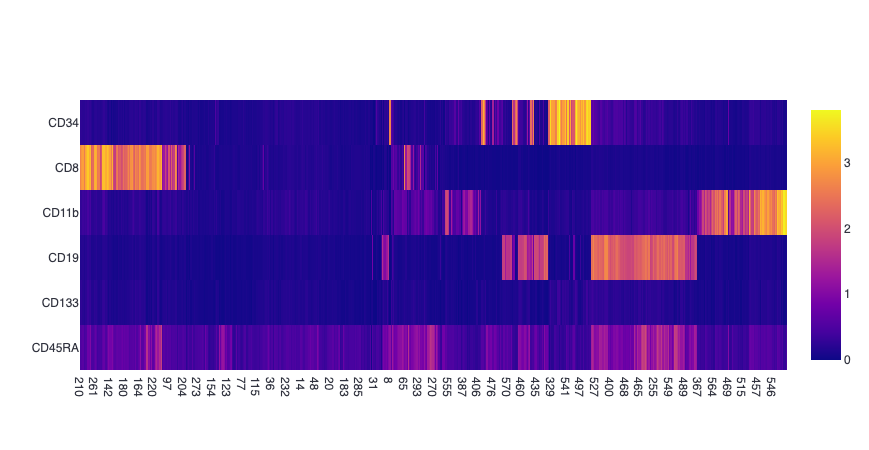
\includegraphics[width=0.9\textwidth]{Figures/heatmapex.png}
        \caption{Heatmap}
        \label{fig:heatmap}
    \end{figure}

    \item 2D exploration of data
    
    The 2D exploration of data offers several options: the selection of two features, scatterplot matrix for all features, and various dimensionality reduction algorithms (PCA, t-SNE, UMAP). The color of each of the datapoints matches the color in the dendrogram. Scatterplot matrix for all features is not recommended for large datasets. 
    
    The PlotMaster searches for data reduction data in the "user\textunderscore data" folder. Should the data not be found it is created by leveraging the sklearn library, and saved in the "user\textunderscore data" folder for later use. 
    
    \begin{figure}[h!]
        \centering
        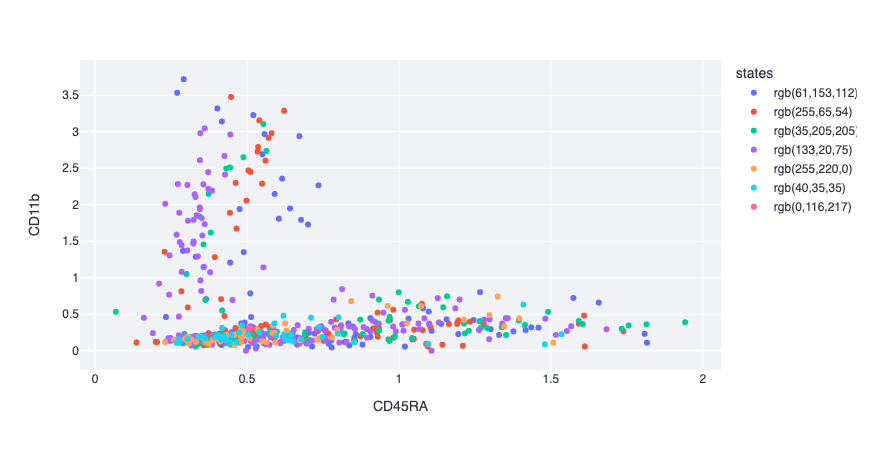
\includegraphics[width=0.9\textwidth]{Figures/twofeat.png}
        \caption{Two Selected Features}
        \label{fig:twofeat}
    \end{figure}

    \item 3D exploration of data
    
    The 3D exploration of data focuses on three dimensionality reduction algorithms: PCA, t-SNE, UMAP. The color of each of the datapoints matches the color in the dendrogram. The user can rotate the plot at will.
    
    The PlotMaster searches for data reduction data in the "user\textunderscore data" folder. Should the data not be found it is created by leveraging the sklearn library, and saved in the "user\textunderscore data" folder for later use. 
    \begin{figure}[h!]
        \centering
        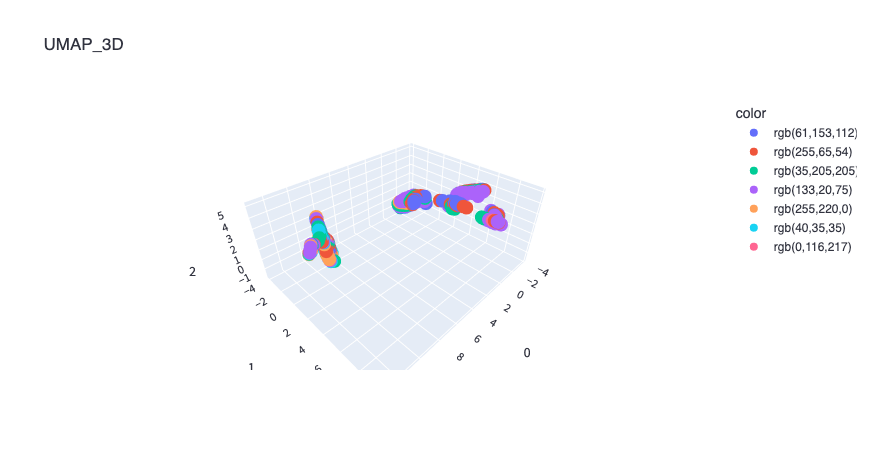
\includegraphics[width=0.9\textwidth]{Figures/umap3d.png}
        \caption{UMAP 3D}
        \label{fig:umap3d}
    \end{figure}
    
\end{itemize}

\newpage
\subsection{User Interface}
\label{sec:userinter}
\paragraph{Streamlit}
\label{sec:st2}
The interface in Streamlit was designed to be simple. Streamlit comes with some formatting out of the box, therefore it is easy to plug it in and have a decent looking application immediately. It also has naive support for Plotly, making it easy to connect the interface to the plotting part of the application. 

For layout, the page configuration was set to wide to make most of users screen's real estate, with two columns. The layout scales with Brave and Chrome browser zoom tool.

On the left, there is a slider, a dropdown menu, and two graph: a dendrogram and a heatmap. The slider is connected to the dendrogram's color threshold, and the user can select any integer from 0 to the maximum value in heights.csv. The dropdown menu allows for selection of multiple values. The values are strings representing features in the dataset. Selected options are plotted in a heatmap, which can be found just under the dendrogram. 

On the right, there is a dropdown menu which allows for selection of multiple options. The offered options are tied to 2D and 3D plots described in \ref{sec:data-plotting}. Plots are displayed in selected order. 

    \begin{figure}[h!]
        \centering
        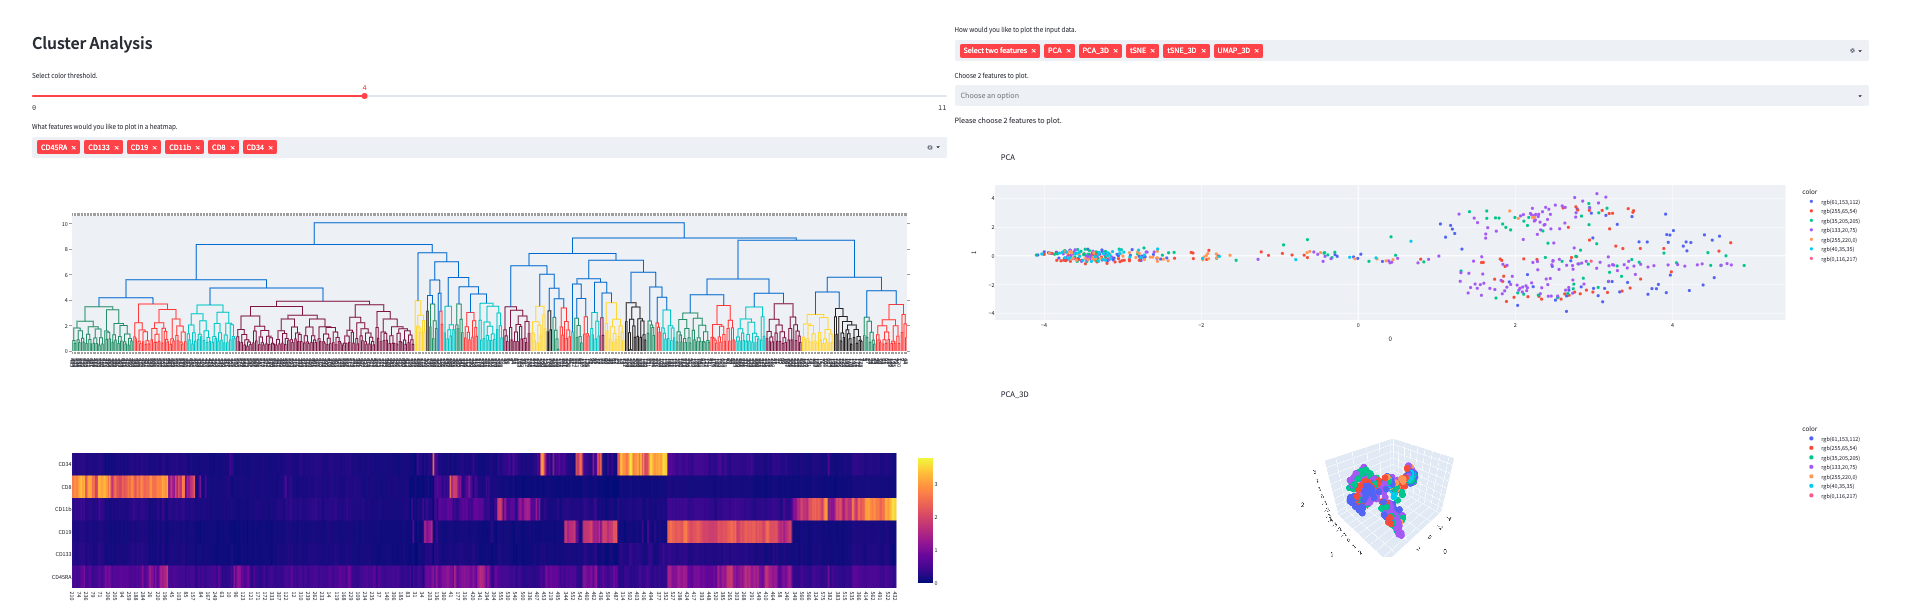
\includegraphics[width=0.9\textwidth]{Figures/streamlit_screen.png}
        \caption{Streamlit Layout}
        \label{fig:streamlay}
    \end{figure}


\newpage
\section{Architecture Challenges}
\label{sec:arch_chal}
\paragraph{Plotly}
\label{sec:plotlych}
Even though Plotly presents itself as a plotting library, it takes care of more than just plotting data. For example, plotly offers a function called create\textunderscore dendrogram, which offers nice tools for working with dendrograms, such as assigning colors, giving reports about each of the leaves, and more. However, the function expects input in the format of raw data, which is incompatible with the input as required from the user (described in \ref{sec:data-parsing}). 

To work around the issue, the function was monkey patched. Monkey patching allows to modify or extend behavior at runtime, eliminating the need to alter the original source code. Thanks to monkey patching the function and underlying Dendrogram class, it was possible to plot the dendrogram data that were obtained from a different algorithm than the one hiding under create\textunderscore dendrogram. 

\paragraph{Streamlit}
\label{sec:st3}
One of the main challenges when working with Streamlit (\ref{sec:streamlit}) is the lack of intelligent interaction with the interactive components provided by the solution. Any time a change is made anywhere, the whole code is rerun, prolonging waiting times for the user. That is also true for components that were not affected by the change. 

Streamlit offers a couple of solutions to the issue. It is recommended to precompute and everything possible, and load the precomputed files into Streamlit instead. 

Another option is to leverage Streamlit's naive cache. The cash promises improved manipulation with large datasets and performing expensive operations. It can be implemented by using the @streamlit.cache decorator on expensive functions. When a function is called with @streamlit.cache decorator, Streamlit checks whether the input parameter has changed, whether any value of any external variable has changed, what is inside the body of the function, and the body of any function called inside the decorated function. Everything is cached the first time the program is run, making the first run more expensive than subsequential runs. 

\paragraph{Dash}
\label{sec:dash3}
A comparable solution was built in Dash, relying on the same PlotMaster background. The lack of out of box formatting was noticable, making the app less pleasant to work with. 

Another challenge was to create a way to share information between each part of the application, since unlike Streamlit, Dash works in a series of callbacks as described in \ref{sec:dash}. Fortunately, Dash offers a data storage components, which enables the communication. 

One of the issues Streamlit brings is that it reruns the whole code whenever anything is changed. It also recomputes all elements that were not subject to the change, making it desirable to implement intermittent data saving and loading to reduce any necessary computation. Streamlit's own caching solution is in development at time of writing this. 

The author found Streamlit's interface easier to navigate by a small margin, and integrated formatting out the box makes the application look more well rounded compared to out of the box bareness of Dash, which expects user specified formatting, ideally in the form of a .css file.
